\documentclass{practicaitic}
\usepackage{parskip}
\usepackage{graphicx}

\usepackage[onelevel]{exercici}
%\usepackage[utf8]{inputenc}

\numpract{1}
\title{Pràctica 1: Posada en marxa d'un VPS}

\assignatura{Aplicacions i Serveis sobre Internet}
\autor{Eric Roy Almonacid \and Francisco del Águila López}

\begin{document}

\section{Introducció}

Aquesta pràctica és l'inici d'un seguit de pràctiques seqüencials, on
l'objectiu final és disposar d'un servidor obert a internet i el coneixement
necessari per poder-hi configurar gairebé tots els serveis \textit{self-hosted}
que hi ha disponibles al mercat.

\subsection{Objectius}

Al finalitzar aquesta pràctica, l'estudiantat haurà:
\begin{enumerate}
  \item Creat un servidor en local o amb un proveïdor de serveis al núvol.
  \item Configurat l'adreçament IPv4 i IPv6 al servidor.
  \item Creat diferents usuaris al servidor amb grups diferents.
  \item Configurat SSH per clau privada.
  \item Connectat el servidor al VPN de l'escola.
\end{enumerate}

\subsection{Condicions}

Aquesta pràctica està cal·librada per ésser treballada en equips de 2 persones,
i té una durada de 2 setmanes.

\subsection{Lliuraments}

S'haurà de realitzar una entrega a Atenea i mantenir operatiu el servidor creat
fins que la pràctica sigui avaluada. El format de la entrega està detallat a
l'apartat \ref{sec:entrega}.

\section{El concepte de VPS}

Hi ha diverses alternatives per poder disposar dels seus propis serveis a
Internet:

\begin{itemize}
  \item Muntar un servidor a casa seva: és una alternativa més econòmica, però
  requereix tenir un ordinador sempre connectat a l'encaminador i una IP pública.
  Actualment molts proveïdors d'internet co\lgem oquen els seus usuaris darrere un
  \textit{Carrier-Grade NAT} (CG-NAT), que els impedeix configurar la
  redirecció de ports de la seva adreça IP pública, ja que és compartida amb la
  resta d'usuaris.
  \item Llogar recursos a tercers: la alternativa més senzilla, ja no ens hem
  de preocupar de tota la part del maquinari.
\end{itemize}

Tanmateix, llogar un servidor sencer no és sempre necessari: sovint amb pocs
recursos ja es pot desplegar serveis com \textit{Moodle}, \textit{Wordpress},
o fins i tot un servidor de \textit{Minecraft}.
Així doncs, per abaratir els preus es poden crear diferents màquines virtuals
en un servidor i llogar cadascuna per separat.

Un \textit{Virtual Private Server} (VPS) és una d'aquestes màquines, amb una
adreça única assignada per fer-la accessible des d'internet. En aquesta
pràctica llogarem i configurarem el nostre primer VPS. Veureu que, a efectes pràctics,
no sabrem que estem treballant sobre una màquina virtual.

\section{Desenvolupament de la pràctica}

La majoria de proveïdors
ofereixen serveis a preus molt baixos i amb períodes de prova molt amplis, però
si ho preferiu podeu realitzar les pràctiques amb un ordinador de casa vostra.

En aquests casos haureu de tenir present els requeriments d'adreça IP i
\textit{uptime} (haurà d'estar sempre accessible), i haureu d'adaptar els
enunciats pel vostre cas particular.

\subsection{Creació del VPS}

Per l'enunciat d'aquesta pràctica hem decidit utilitzar com a exemple el
proveïdor \textit{Hetzner} per la seva simplicitat i preu. Tanmateix,
qualsevol que ofereixi un VPS amb IPv4 i
IPv6 públiques haurien de servir (OVH, DigitalOcean, ...).

En el cas de \textit{Hetzner}, es poden compartir enllaços d'afiliat o trobar
codis de descompte a la seva pàgina web per gaudir de 3 mesos de prova. Per
exemple, a la part dreta de qualsevol article de \url{https://community.hetzner.com} hi ha un
codi de descompte.

\begin{tasca}
Creeu-vos un compte a \url{https://accounts.hetzner.com/signUp} i
verifiqueu-lo introduint un mètode de pagament. Si utilitzeu un altre proveïdor,
indiqueu-ho en l'entrega.
\end{tasca}

\begin{previ}
Aneu a \url{https://console.hetzner.cloud} i creeu un nou projecte, i
llavors un nou servidor a dintre d'aquest. Com a imatge base us
recomanem utilitzar la darrera versió de Debian. Agafeu l'arquitectura i
recursos més econòmics, i la majoria d'opcions poden ser per defecte.
Anoteu-vos l'adreça IPv4 i IPv6 del servidor.
\end{previ}

Un cop en marxa el servidor, hauríeu de veure quelcom similar a la Figura \ref{fig:h1}.

\begin{figure}[h]
  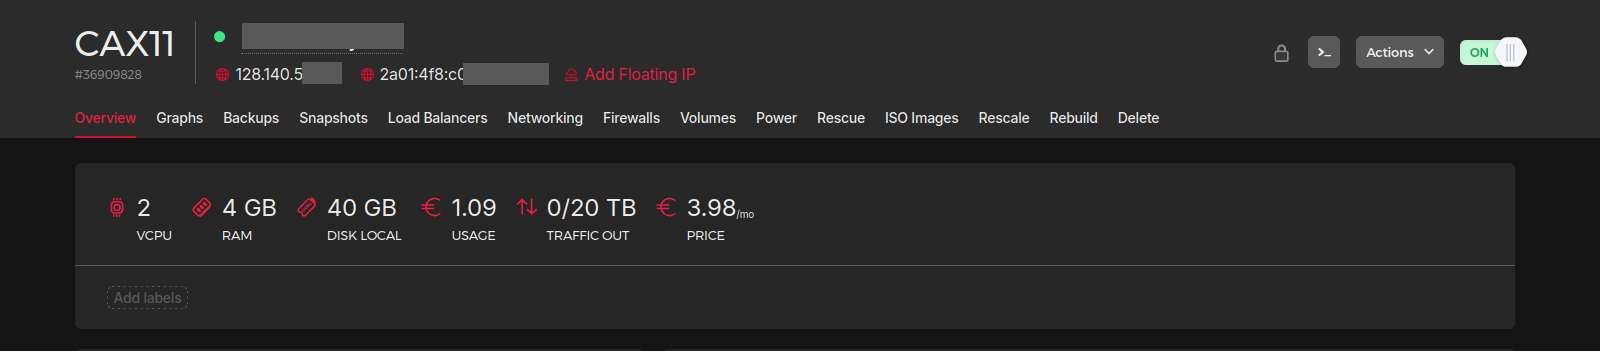
\includegraphics[width=0.9\linewidth]{assets/hetzner1.png}
  \centering
  \label{fig:h1}
  \caption{Tauler de control del servidor a \textit{Hetzner}.}
\end{figure}

\subsubsection{Accedir al servidor}

En la majoria de VPS podreu preconfigurar bastantes coses (usuaris, servei SSH),
però partirem des de zero. Un cop creat el servidor accedirem a la consola,
on veurem que només hi ha un usuari inicial (root).

\begin{previ}
Accediu a la consola del servidor i comproveu que podeu interactuar amb
ell. Des de la Figura \ref{fig:h1} es pot accedir a la consola a partir de la
icona \verb|[>_]|, a la dreta del tot. Si desconeixeu la contrasenya de
l'usuari \verb|root| la podeu tornar a generar a la pestanya de \textit{Rescue}.
\end{previ}

\subsubsection{Configuració de xarxa}

Per defecte, si executeu \texttt{ip a} al servidor hauríeu de poder veure
que a l'interfície corresponent ja hi té configurada l'adreça, i gràcies a
això el VPS es pot connectar a internet. Tanmateix, alguns proveïdors no configuren
l'adreçament IPv6. En el cas de \textit{Hetzner}, aquest assigna un rang de IPv6
per cada VPS. Haureu d'escollir una adreça d'aquest rang i assignar-la a la màquina.

\begin{previ}
A partir dels coneixements adquirits a Xarxes de Computadors, assegureu-vos
que el VPS té adreçament IPv4 i IPv6. Podeu utilitzar l'eina \texttt{ping} per comprovar
que els paquets arriben al servidor.
\end{previ}

\subsubsection{Configuració del tallafocs}

% Hi ha possibilitat de crear tallafocs a dins o està bloquejat? En
% realitat és un VPS tipus LXC o Docker? on no es pot tocar el kernel?

La majoria de proveïdors de VPS ofereixen la possibilitat de desplegar un
tallafocs o \textit{firewall} a fora del servidor. Al no poder modificar el tallafocs
des de l'interior del servidor, això suposa una barrera addicional en la seguretat
de la màquina. \textit{Hetzner} ofereix aquesta possibilitat: es pot configurar
a partir de la pestanya \textit{Firewall} de la Figura \ref{fig:h1}.

\begin{previ}
Configureu, si podeu, el tallafocs del vostre proveïdor per acceptar només
els paquets ICMP (ping), i de SSH (port 22/tcp). Si l'activeu, haureu de pensar més endavant en
afegir excepcions pels serveis que anirem creant.

Podeu comprovar el funcionament del tallafocs intentant-vos connectar al
servidor al port 22 i a un altre port mitjançant \textit{netcat}:
\begin{itemize}
\item Servidor:
\begin{verbatim}
  nc -l -p <port> -vv
\end{verbatim}
\item Client:
\begin{verbatim}
  nc <ip_del_servidor> <port> -vv
\end{verbatim}
\end{itemize}
  
Observeu el correcte funcionament del tallafocs. Proveu també de fer
\texttt{ping} al servidor.
\end{previ}

\subsection{Creació d'usuaris}

Al tenir un servidor obert a Internet és crucial protegir-lo des d'un primer
moment. El primer pas que farem serà crear usuaris per no treballar sempre
amb \texttt{root}.

Recordeu que per afegir un usuari \texttt{pepito} que, a part d'estar dins del
grup \texttt{pepito}, també estigui al grup \texttt{epsem}, la comanda a executar
seria la següent (amb la darrera comanda crearíem una contrasenya per l'usuari):
\begin{verbatim}
adduser pepito
usermod -aG epsem pepito
passwd pepito
\end{verbatim}

\begin{previ}
Creeu tres nous usuaris al servidor:
\begin{itemize}
  \item Un per cada integrant del grup. Per exemple \texttt{eric} i \texttt{paco}.
  \item Un altre anomenat \texttt{profe} amb el que els professors es connectaran
  per revisar el servidor.
\end{itemize}
Afegiu al grup \texttt{sudo} els tres usuaris, i creeu una contrasenya per
cada un d'ells.
\end{previ}

\subsection{Configuració de SSH}

Com us podeu imaginar, no és molt pràctic treballar al servidor des de la
interfície del navegador. SSH o \textit{Secure SHell} és un protocol que permet
accedir a la consola d'un ordinador remotament. Anem a configurar-lo pel nostre
servidor. Necessitareu el paquet \texttt{openssh-server} al servidor, i \texttt{ssh}
al vostre ordinador (tot i que segurament ja els teniu insta\l.lats).

\begin{previ}
Executeu \texttt{systemctl start sshd} per engegar el servidor \textit{ssh}.
\end{previ}

Fent \texttt{ssh -p port usuari@ip\_del\_servidor} des del vostre
ordinador, executareu el client per connectar-vos remotament al
servidor. El port es pot ometre si és el per defecte (22), i l'usuari
es pot ometre si és el mateix que el del vostre ordinador.

\begin{previ}
Podeu connectar-vos amb l'usuari \textit{root} al servidor mitjançant SSH?
Això no és una bona pràctica de seguretat. Modifiqueu el fitxer \texttt{/etc/ssh/sshd\_config},
i canvieu \texttt{PermitRootLogin} de \verb|yes| a \verb|no|.

Guardeu el fitxer i
reinicieu el servei de SSH mitjançant \texttt{systemctl restart sshd}. Comproveu que
ja no podeu connectar-vos amb \texttt{root}.

Aprofiteu per fer una ullada al fitxer de configuració. Potser us pot interessar
fer algun canvi més.
\end{previ}

\subsubsection{Accés amb claus asimètriques}

Actualment, l'únic que protegeix el vostre servidor d'un atac és la
contrasenya del vostre usuari. Això és vulnerable a atacs de força
bruta per contrasenyes febles a part que el mecanisme
\texttt{usuari/contrasenya} és més vulnerable degut a que escriure-la
contínuament permet que sigui interceptada. SSH ofereix com a
alternativa l'autentificació per claus asimètriques.

\begin{previ}
Genereu un parell de claus asimètriques. Cada integrant del grup ha de
generar les seves. Us recomanem utilitzar RSA de 4096 bits.

Podeu consultar el manual de \texttt{ssh-keygen} tant amb la comanda
\texttt{man} com a \url{https://www.ssh.com/academy/ssh/keygen}.
\end{previ}

Aquest procediment regenera un parell de claus, una pública i una altra
privada. A priori, la clau privada es queda en el dispositiu on s'han
generat el parell de claus (Client) des d'on s'executarà la comanda
\texttt{ssh}. La clau pública generada es pot anar replicant en cada
Servidor on es requereixi l'autentificació del Client. Cal remarcar,
que cada parell de claus està associat a l'usuari que les ha generat.

Es donarà accés al servidor als professors. A Atenea trobareu penjada
una clau pública que haureu d'afegir a l'usuari \texttt{profe}. Els professors
utilitzaran aquest accés només per avaluar les pràctiques, i no modificaran
l'estat del servidor.

El següent pas
és posar les 3 claus públiques al servidor.

\begin{previ}
Copieu la clau pública de cada integrant al fitxer
\texttt{/home/<USUARI>/.ssh/authorized\_keys}. Cada usuari té un fitxer diferent,
i pot tenir diferents claus (1 per línia), representant diferents dispositius.
\end{previ}

Ara només faltarà deshabilitar les connexions per contrasenya. Abans,
però, us recomanem comprovar que us podeu connectar sense posar
contrasenya. Si podeu, significa que SSH ha reconegut el procediment
amb clau asimètrica (pública i privada) i podeu seguir sense tenir por
de quedar-vos sense accés al servidor.

\begin{previ}
Deshabiliteu les connexions SSH per contrasenya i reinicieu \texttt{openssh}.
Haureu de modificar el mateix fitxer que abans.

Ara no hauríeu de poder connectar-vos des de l'ordinador d'un altre company
de classe (que no té la vostra clau privada), però sí des del vostre.
\end{previ}

\section{Connexió al VPN de l'escola}

Per poder connectar-se fàcilment als servidors de la resta de grups i
poder seguir correctament les pràctiques posteriors farà falta
connectar el VPS a la VPN \emph{Virtual Private Network} de l'Escola,
creada amb OpenVPN per a aquesta assignatura.

\begin{previ}
  Connecteu-vos al servidor VPN de l'escola amb el vostre servidor.
  Assigneu la IP \texttt{172.20.ng.2} a la interfície que creareu, on $ng$ és
  el vostre número de grup.

  Per realitzar aquesta tasca us serà útil llegir l'apartat 5.1 de l'enunciat de
  la versió alternativa d'aquesta pràctica, disponible a l'OpenCourseWare.
\end{previ}

Finalment, podeu comprovar l'accés a través del VPN, connectant-vos a
la VPN amb el vostre ordinador personal (assigneu una alta adreça IP,
per exemple \texttt{172.20.ng.3}). Tenint en compte que el vostre VPS
ja té accés a la VPN (tasca anterior), proveu de comprovar la
connectivitat amb un \texttt{ping} des del vostre ordinador personal
utilitzant l'adreça IP \texttt{172.20.ng.2} enlloc de l'adreça
pública.

\section{Avaluació}

Aquest apartat detalla com s'ha d'entregar i avaluar la pràctica.

\subsection{Entrega}
\label{sec:entrega}

S'ha d'entregar un fitxer compactat amb formats lliures (\texttt{P1\_GX.ext}, on X és el número o 
lletra del grup i \emph{ext} és l'extensió del compactador) que contingui un fitxer de text amb el següent format:

\begin{verbatim}
Grup: GX
IPv4: 128.140.55.126
IPv6: 2a01:4f8:c013:7f5::1
Contrasenya usuari profe: Lkv5YYyON8X
Port SSH: 22

(Comentaris referents a l'entrega, si s'escau)
\end{verbatim}

Evidentment, heu de posar els valors del vostre servidor i grup.

Al servidor, creeu el directori
\texttt{/entregues} a l'arrel, i a dins un directori
\texttt{/entregues/p1}. Allà hi heu de deixar els scripts i/o manuals
(el que cregueu convenient) que us farien falta si mai haguéssiu de
repetir aquesta pràctica. Incorporeu també aquesta informació al lliurament.

Per exemple, podríeu indicar:
\begin{itemize}
  \item El proveïdor que heu utilitzat, els seus preus i ofertes, i el perquè l'heu escollit.
  \item Solucions a problemes que us heu trobat, i si cal, enllaços a fòrums o manuals.
  \item Comandes que heu utilitzat amb una petita explicació de què fan (1 línia sol ser suficient).
  \item Altres coses que hagueu fet (per exemple, configurar el tallafocs de \textit{Hetzner}).
\end{itemize}

No ha de ser extens, aquests documents us serviran a vosaltres si mai heu de
crear un servidor nou.

%\newpage % Sinó queda el títol i una línia sola
\subsection{Qualificació}

Aquesta pràctica per considerar-se fonamental pel desenvolupament de
les següents pràctiques no tindrà avaluació, de la mateixa manera que
la seva alternativa amb màquines virtuals locals. Però a mode de
rúbrica (criteri de valoració) disposeu de la següent taula. La
puntuació màxima és 100.

\begin{center}
  \begin{tabular}{ll}
  \hline
  Concepte & Rang \\ \hline
  Fitxer de l'entrega (\texttt{P1\_GX.ext}) amb format correcte & $[-20, 0]$ \\
  Es pot fer ping al servidor per IPv4 & $[0, 5]$ \\
  Es pot fer ping al servidor per IPv6 & $[0, 5]$ \\
  SSH amb contrasenya o amb root habilitat & $[-10, 0]$ \\
  El servidor té usuaris per cada integrant i usuari \texttt{profe} & $[0, 10]$ \\
  Es pot fer SSH al servidor amb la clau privada de \texttt{profe} & $[0, 20]$ \\
  L'usuari \texttt{profe} no pot fer \texttt{sudo} & $[-10,0]$ \\
  El servidor està connectat al VPN de l'escola & $[0, 20]$ \\
  Qualitat dels scripts/tutorials de \texttt{/entregues/p1} & $[0,40]$ \\
  El servidor presenta problemes de seguretat greus & $[-10,0]$ \\
  \hline
  \end{tabular}
\end{center}

Nota: si el vostre proveïdor no us permet tenir una adreça IPv6 pública
indiqueu-ho als comentaris del fitxer de la entrega. En aquest cas, l'apartat
sobre IPv4 valdrà el doble i el de IPv6 queda a zero.

Tingueu present que si algun element de la taula anterior no es pot avaluar
(per exemple, al no poder fer \texttt{sudo} no es pot llegir els continguts de \texttt{/entregues/p1})
aquest es qualificarà amb la nota més baixa.

Si es detecta algun tipus de frau en l'entrega aquesta rebrà una puntuació de zero.

\end{document}
